%-------------------------------------------------------
% Discussion.tex
%
% This document contains the discussion about SDN and
% OpenFlow security of the paper
%-------------------------------------------------------
\section*{\small\textsc{III. security analysis}}
The basic properties of a secure communications network are: confidentiality, integrity, availability of information, authentication and non repudiation. If one or more properties miss the communication can not be considered secure.
\ac{SDN} and OpenFlow are developed with the main goal to reach the market soon as possible. Indeed both \ac{SDN} and OpenFlow suffer for some security problem.

\subsection*{\raggedright\small\textit{A. Weaknesses}}
\ac{SDN} and OpenFlow offers many benefits in network management but exposes new attack points that can be exploited by an attacker; the most important are the \ac{CP} and the OpenFlow communication protocol itself, in addition to the old attack points like routers and switches with they're weakness.

The \ac{SDN} architecture simplifies the hardware operations but it also brings single point security issues: once the controller is attacked, all low level switches are mislead and cannot correctly deliver the packets.

In \cite{acm:openflow-weakness} the authors show two critical points. First, an attacker could exploit the bottleneck, that arises between the \ac{CP} and \ac{DP}, by mounting a \attack{\acf{CP} saturation attack} that disrupts network operations. Second, an attacker could enabling the \ac{CP} to expedite both detection of, and responses to, the changing flow dynamics with the \ac{DP}.

Another major problem, discussed in \cite{onf:openflow-specifications}, is to consider secure the communication channel between the \ac{CP} and \ac{DP}. The OpenFlow switch specifications describe the use of \ac{TLS} with the mutual authentication between the controllers and the switches. However, this security features is optional, and the standard of \ac{TLS} is not specified. The lack of \ac{TLS} adoption by major routers/switches vendors and the possibility of \attack{\ac{DoS} attacks} are the focus of an OpenFlow vulnerability assessment \cite{acm:openflow-tls-vulnerability}. The authors found that the lack of \ac{TLS} use could lead to fraudulent rule insertion or modification.

\section*{\small \textsc{security enhancement using \ac{SDN}}}
The architecture of \ac{SDN} introduces potential for innovation in the use of the network. The combination of the global view of the network and the network programmability supports process of harvesting intelligence informations from existing \ac{IDS} and \ac{IPS}. For example, followed by analysis of \ac{IDS}/\ac{IPS} the \ac{CP} can reprogramming the network policy. This approach can render the \ac{SDN} more robust to malicious attack than traditional network.

The necessity of a different way to do inspection is motivated by the conventional regimes do not work very well in cloud data centres. In \cite{sdn-and-openflow-from-concept-to-implementation:NICE} they talk about a module called \ac{NICE} running on each server with a low overhead. This module is composed by two phases: (a) \ac{NICE}-A and (b) \ac{DPI}. The \ac{NICE}-A phase is an agent intrusion detection that scan and update the \ac{SAG}. The \ac{DPI} phase is activated when the \ac{VM} enters in ``inspection state'' and use the \ac{SAG} to found imminent threat and vulnerabilities.

The \ac{SDN} architecture simplifies the hardware operations but it also brings single point security issues: once the controller is attacked, all low level switches are mislead and cannot correctly deliver the packets. To solve this threat, in \cite{fresco-services} authors introduces a security application development framework. The framework, shown in Figure \ref{fig:security-enhancement-using-SDN:FRESCO},

\begin{figure}
\centering
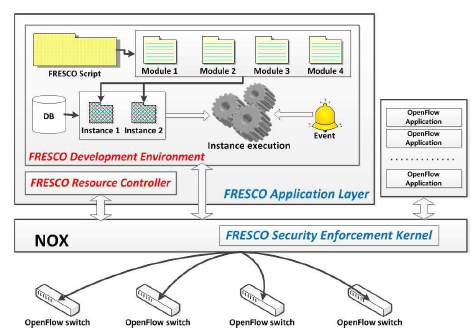
\includegraphics[scale=0.5]{Introduction/Image/FrescoStructure.png}
\caption{FRESCO: a high level overview}
\label{fig:security-enhancement-using-SDN:FRESCO}
\end{figure}

is composed by 16 libraries that allow the users write security application. It execute operation like: simple block of addresses or dynamic quarantine or reflect remote scanner in a ``honey net''. The reasons that led to the birth of FRESCO are three. The first is a concept known as ``\ac{IDC}'', the controllers do not track information for network security but FRESCO has a \ac{DB} for such data. Second incorporates an architectural design that is modular inspired by the click router. Finally product some alerts in response of a malicious combination of network flow.

In \cite{sdn-anomaly-traffic-detection} the authors propose different OpenFlow algorithm for anomaly traffic detection. They evaluate all the algorithm in home and business networks. In the following I summarize their ideas. The first algorithm proposed is called \ac{TRW-CB}. In accordance with a \ac{TCP} connection can be established in a much higher success rate if the server is not attacked. Using sequential hypothesis (i.e. likelihood ratio test), the analyses each connection status and attempt to detect the worm infections. A second algorithm exposed is called \ac{RL}. A virus infection can cause many connection request within very short time, while a benign flow traffic flow will never have such a high request rate. This is the principle of \ac{RL}, that is, to check the request rate and  detect malicious events. The third algorithm exposed is called \ac{MED}. The entropy calculations can be used to find traffic statistic features. By using a baseline distribution, maximum entropy model can be used to classify the packets into different categories, and each category could be detected as benign or malicious. The last algorithm exposed is called \ac{NETAD} and acts like a firewall or filter. It simply scan the packet header and blocks any suspicious packet based on the packet attributions.